% ============================================================
%  Minimal Beamer Template — Nord Color Theme
%  Nord palette: https://www.nordtheme.com/
% ============================================================
\documentclass[aspectratio=169]{beamer}

% ---------- packages ----------------------------------------
\usepackage[T1]{fontenc}
\usepackage[utf8]{inputenc}
\usepackage{lmodern}
\usepackage{xspace}
\usepackage{microtype}
\usepackage{booktabs}
\usepackage{graphicx}
\usepackage{tikz}
\usetikzlibrary{arrows.meta, positioning, shapes.geometric}

% ============================================================
%  Nord Color Definitions
% ============================================================
%  Polar Night
\definecolor{nord0}{HTML}{2E3440}
\definecolor{nord1}{HTML}{3B4252}
\definecolor{nord2}{HTML}{434C5E}
\definecolor{nord3}{HTML}{4C566A}
%  Snow Storm
\definecolor{nord4}{HTML}{D8DEE9}
\definecolor{nord5}{HTML}{E5E9F0}
\definecolor{nord6}{HTML}{ECEFF4}
%  Frost
\definecolor{nord7}{HTML}{8FBCBB}
\definecolor{nord8}{HTML}{88C0D0}
\definecolor{nord9}{HTML}{81A1C1}
\definecolor{nord10}{HTML}{5E81AC}
%  Aurora
\definecolor{nord11}{HTML}{BF616A}  % red
\definecolor{nord12}{HTML}{D08770}  % orange
\definecolor{nord13}{HTML}{EBCB8B}  % yellow
\definecolor{nord14}{HTML}{A3BE8C}  % green
\definecolor{nord15}{HTML}{B48EAD}  % purple

% ============================================================
%  Beamer Theme Settings
% ============================================================
\usetheme{default}
\useinnertheme{circles}

% --- colors -------------------------------------------------
\setbeamercolor{normal text}        {fg=nord6,  bg=nord0}
\setbeamercolor{alerted text}       {fg=nord11}
\setbeamercolor{example text}       {fg=nord14}

\setbeamercolor{structure}          {fg=nord8}

\setbeamercolor{frametitle}         {fg=nord6,  bg=nord1}
\setbeamercolor{framesubtitle}      {fg=nord4}

\setbeamercolor{title}              {fg=nord6,  bg=nord0}
\setbeamercolor{subtitle}           {fg=nord8}
\setbeamercolor{author}             {fg=nord4}
\setbeamercolor{date}               {fg=nord4}
\setbeamercolor{institute}          {fg=nord14}

\setbeamercolor{footline}           {fg=nord15,  bg=nord1}
\setbeamercolor{headline}           {fg=nord3,  bg=nord1}

\setbeamercolor{block title}        {fg=nord6,  bg=nord2}
\setbeamercolor{block body}         {fg=nord5,  bg=nord1}
\setbeamercolor{block title alerted}{fg=nord6,  bg=nord11}
\setbeamercolor{block body alerted} {fg=nord6,  bg=nord2}
\setbeamercolor{block title example}{fg=nord6,  bg=nord14}
\setbeamercolor{block body example} {fg=nord6,  bg=nord2}

\setbeamercolor{item}               {fg=nord8}
\setbeamercolor{subitem}            {fg=nord9}
\setbeamercolor{subsubitem}         {fg=nord10}

\setbeamercolor{caption name}       {fg=nord8}
\setbeamercolor{button}             {fg=nord6,  bg=nord10}

% --- fonts --------------------------------------------------
\setbeamerfont{title}           {size=\Large,  series=\bfseries}
\setbeamerfont{subtitle}        {size=\normalsize, series=\normalfont}
\setbeamerfont{frametitle}      {size=\large,  series=\bfseries}
\setbeamerfont{framesubtitle}   {size=\small}
\setbeamerfont{footline}        {size=\tiny}

% --- remove nav symbols -------------------------------------
\setbeamertemplate{navigation symbols}{}

% --- frametitle ---------------------------------------------
\setbeamertemplate{frametitle}{%
  \vspace{0.4em}%
  \insertframetitle%
  \ifx\insertframesubtitle\empty\else%
    \\[0.1em]{\usebeamerfont{framesubtitle}\usebeamercolor[fg]{framesubtitle}\insertframesubtitle}%
  \fi%
  \vspace{0.2em}%
}

% --- title page ---------------------------------------------
\defbeamertemplate*{title page}{nord}{%
  \begin{tikzpicture}[remember picture, overlay]
    % accent bar on the left
    \fill[nord10] (current page.north west)
      rectangle ([xshift=0.45cm] current page.south west);
    % frost accent line under title area
    \fill[nord8] ([yshift=-0.38\paperheight] current page.north west)
      rectangle ([xshift=0.45cm, yshift=-0.40\paperheight] current page.north west);
  \end{tikzpicture}%
  \vspace{2em}%
  \begin{beamercolorbox}[sep=0pt, left, leftskip=1cm]{title}
    {\usebeamerfont{title}\usebeamercolor[fg]{title}\inserttitle\par}%
    \vspace{0.4em}%
    {\usebeamerfont{subtitle}\usebeamercolor[fg]{subtitle}\insertsubtitle\par}%
    \vspace{1.2em}%
    {\usebeamerfont{author}\usebeamercolor[fg]{author}\insertauthor\par}%
    \vspace{0.2em}%
    {\usebeamerfont{institute}\usebeamercolor[fg]{institute}\insertinstitute\par}%
    \vspace{0.2em}%
    {\usebeamerfont{date}\usebeamercolor[fg]{date}\insertdate\par}%
  \end{beamercolorbox}%
}

% --- footline -----------------------------------------------
\setbeamertemplate{footline}{%
  \begin{beamercolorbox}[wd=\paperwidth, ht=2.4ex, dp=1.2ex]{footline}%
    \hspace{1em}%
    \usebeamerfont{footline}%
    \insertshortauthor\hfill\insertshorttitle\hfill%
    \insertframenumber\,/\,\inserttotalframenumber\kern1em%
  \end{beamercolorbox}%
}

% --- section page -------------------------------------------
\AtBeginSection[]{%
  \begin{frame}[plain]
    \begin{tikzpicture}[remember picture, overlay]
      \fill[nord1] (current page.south west) rectangle (current page.north east);
      \fill[nord10] ([xshift=-0.5pt] current page.west)
        ++(-2pt,0) rectangle ++(6pt, \paperheight);
    \end{tikzpicture}
    \vfill
    \hspace{1.5cm}%
    \begin{beamercolorbox}[sep=0pt]{title}
      {\color{nord3}\small\MakeUppercase{Section \thesection}}\\[0.4em]
      {\usebeamerfont{title}\color{nord6}\insertsectionhead}
    \end{beamercolorbox}
    \vfill
  \end{frame}%
}

% ============================================================
%  Document Metadata
% ============================================================
\title{Recursive Embedding in Literature}
% \subtitle{An optional subtitle}
\author{Jay Ser}
% \institute{Your Institution}
\date{\today}

 
% ============================================================
% Commands 
% ============================================================
\graphicspath{{./img/}}
\newcommand{\spk}[1]{\makebox[1em][l]{\textbf{#1:}}}

% ============================================================
%  Document
% ============================================================
\begin{document}

\begin{frame}[plain]
  \titlepage
\end{frame}

\begin{frame}{Questions to Keep in Mind}
  \begin{itemize}
    \item Is everything syntax?
    \item ``Rapid fading" design feature of language (Hockett)
    \item Consider an arbitrary ABBA structure in literature.
      Is there a dependency between \textbf{(a)} the corresponding
      opening and closing letters and \textbf{(b)} the embedded inner
      structure and the framing outer structure?
  \end{itemize}

  \medskip
  \begin{columns}[T]
    \begin{column}{0.48\textwidth}
      In discourse (Legate): \\ 
      \noindent\spk{A} Do you carry Michelob?\\
      {\setlength{\hangindent}{3.5em}\noindent\hspace{1.5em}\spk{B} [\textit{sees A has a wet umbrella}] Is it still raining?\par}
      \hspace{1.5em}\spk{A} Yes, unfortunately.\\
      \noindent\spk{B} It's over there, near the plastic cups.
    \end{column}

    \begin{column}{0.48\textwidth}
      In human activity (Pulvermiller, Moro): \\
      \textit{\noindent open the door\\
      \hspace{1.5em} open the bottle\\
      \hspace{1.5em} close the bottle\\
    \noindent close the door}
    \end{column}
  \end{columns}
\end{frame}

\begin{frame}{Ring Composition}
  \begin{columns}[c]
    \begin{column}{0.55\textwidth}
      \begin{figure}
        \centering
        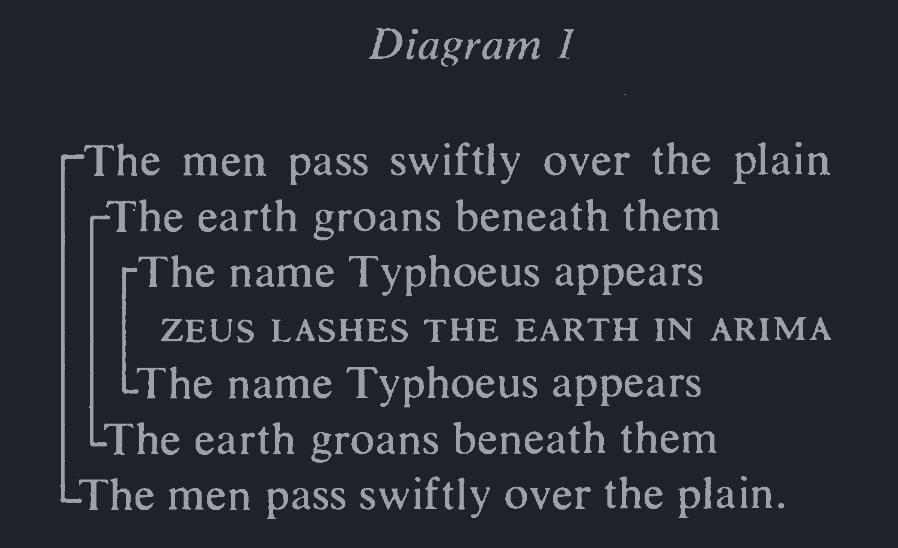
\includegraphics[width=\textwidth]{niles_diag1}
        \caption{Sentential(?) ring composition in the Iliad (Niles)}
      \end{figure}
    \end{column}

    \begin{column}{0.42\textwidth}
      \textit{So the men went, as if the whole earth were being consumed by fire;
      and the earth groaned beneath them, as when Zeus the Thunderer lashes the earth about Typhoeus in anger, in Arima, where Typhoeus is said to lie 
      --- so greatly did the earth groan beneath the feet of the men as they walked, and swiftly they passed over the plain.}
    \end{column}
  \end{columns}
\end{frame}

\begin{frame}{Ring Composition: \textit{Beowulf}} 
  \begin{columns}[c] 
    \begin{column}{0.50\textwidth}
      \centering
      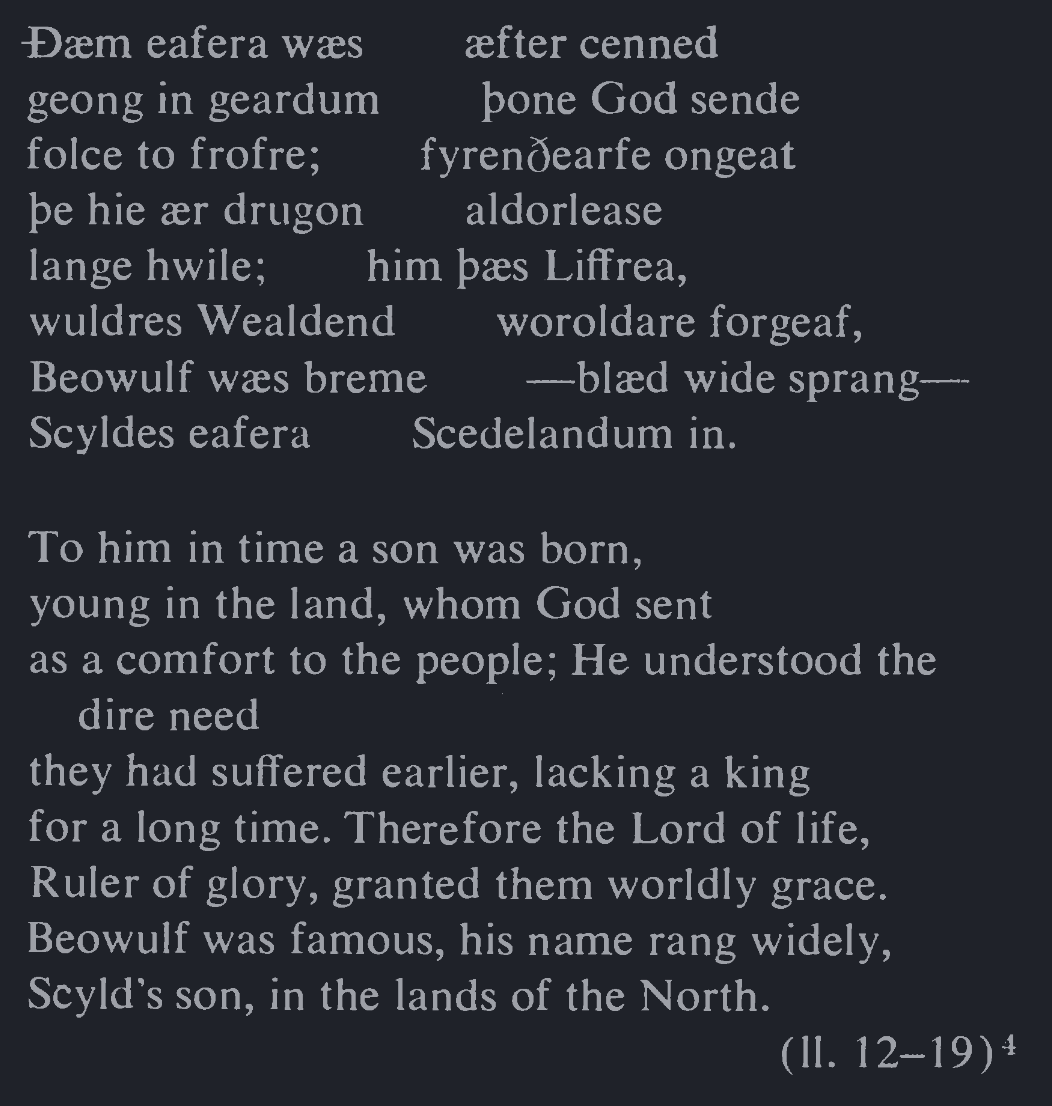
\includegraphics[width=\textwidth]{niles_bw1} 
    \end{column}
    \begin{column}{0.50\textwidth} 
      ``... the poet uses ring composition as a means of traveling from the immediate reality... to an `other,' legendary reality, which is used as a point of comparison..., then  back again to the present. \\ 
      ``Just as the monster Typhoeus is `chained' between balanced links of transitional verse, the Danes's previous sufferings are enclosed safely within the envelope of God's mercy" (Niles). 
    \end{column}
  \end{columns}
\end{frame}

\begin{frame}{Ring Composition: \textit{Beowulf}} 
  \begin{columns}[c]     
    \begin{column}{0.50\textwidth}
      \centering
      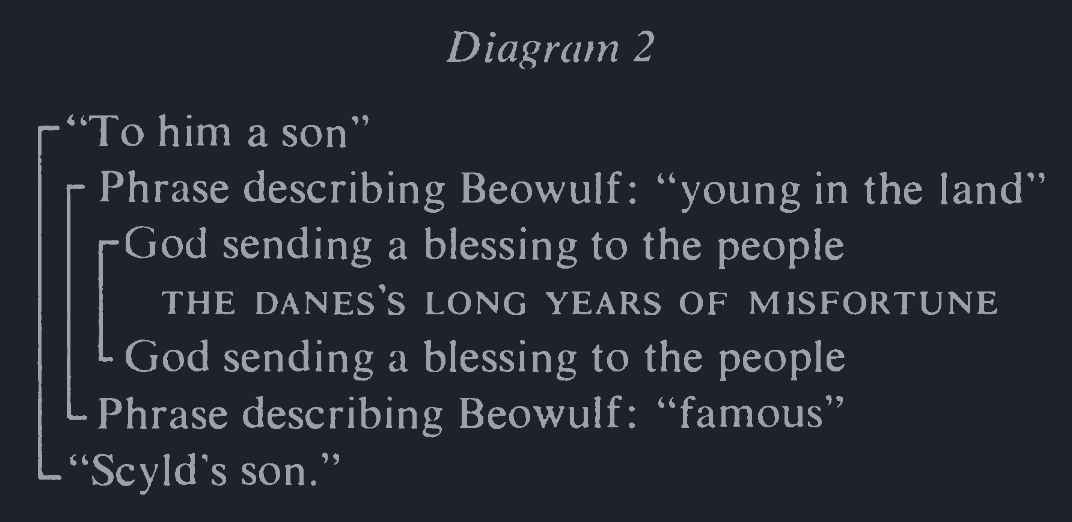
\includegraphics[width=\textwidth]{niles_diag2} 
    \end{column}

    \begin{column}{0.50\textwidth}
      \centering
      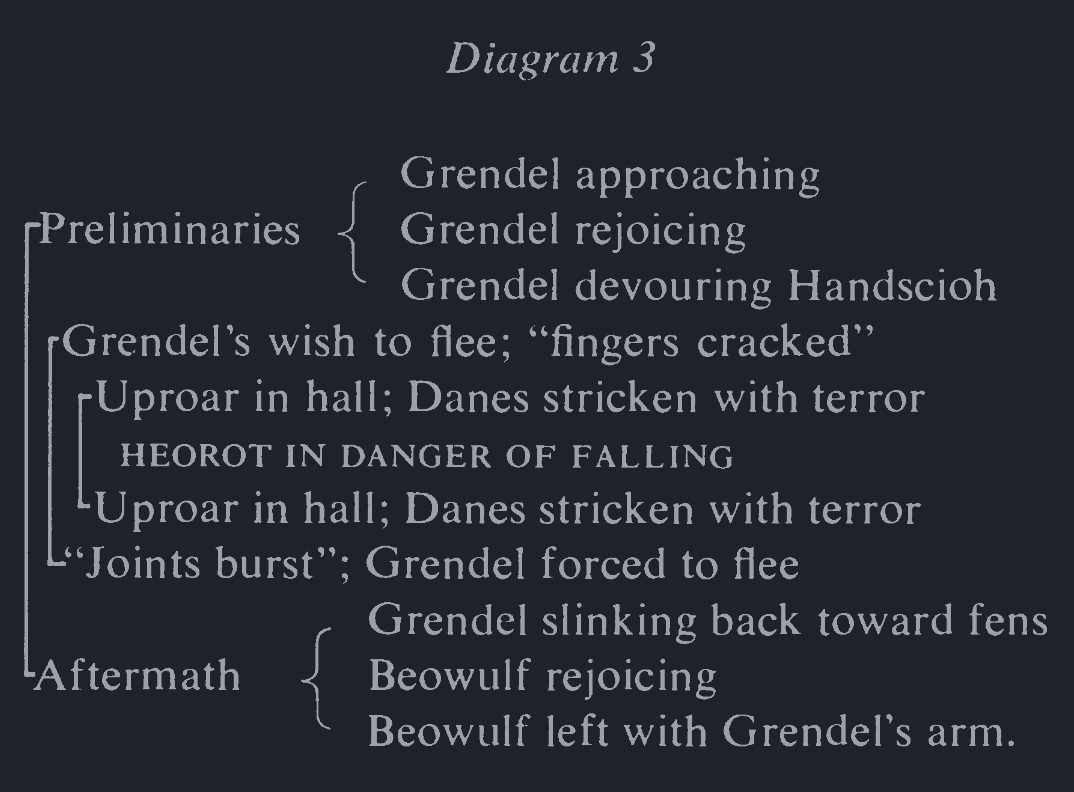
\includegraphics[width=\textwidth]{niles_diag3} 
    \end{column}
  \end{columns}
\end{frame}

\begin{frame}{Ring Composition: \textit{Beowulf}} 
  \begin{columns}[c]     
    \begin{column}{0.38\textwidth}
      \centering
      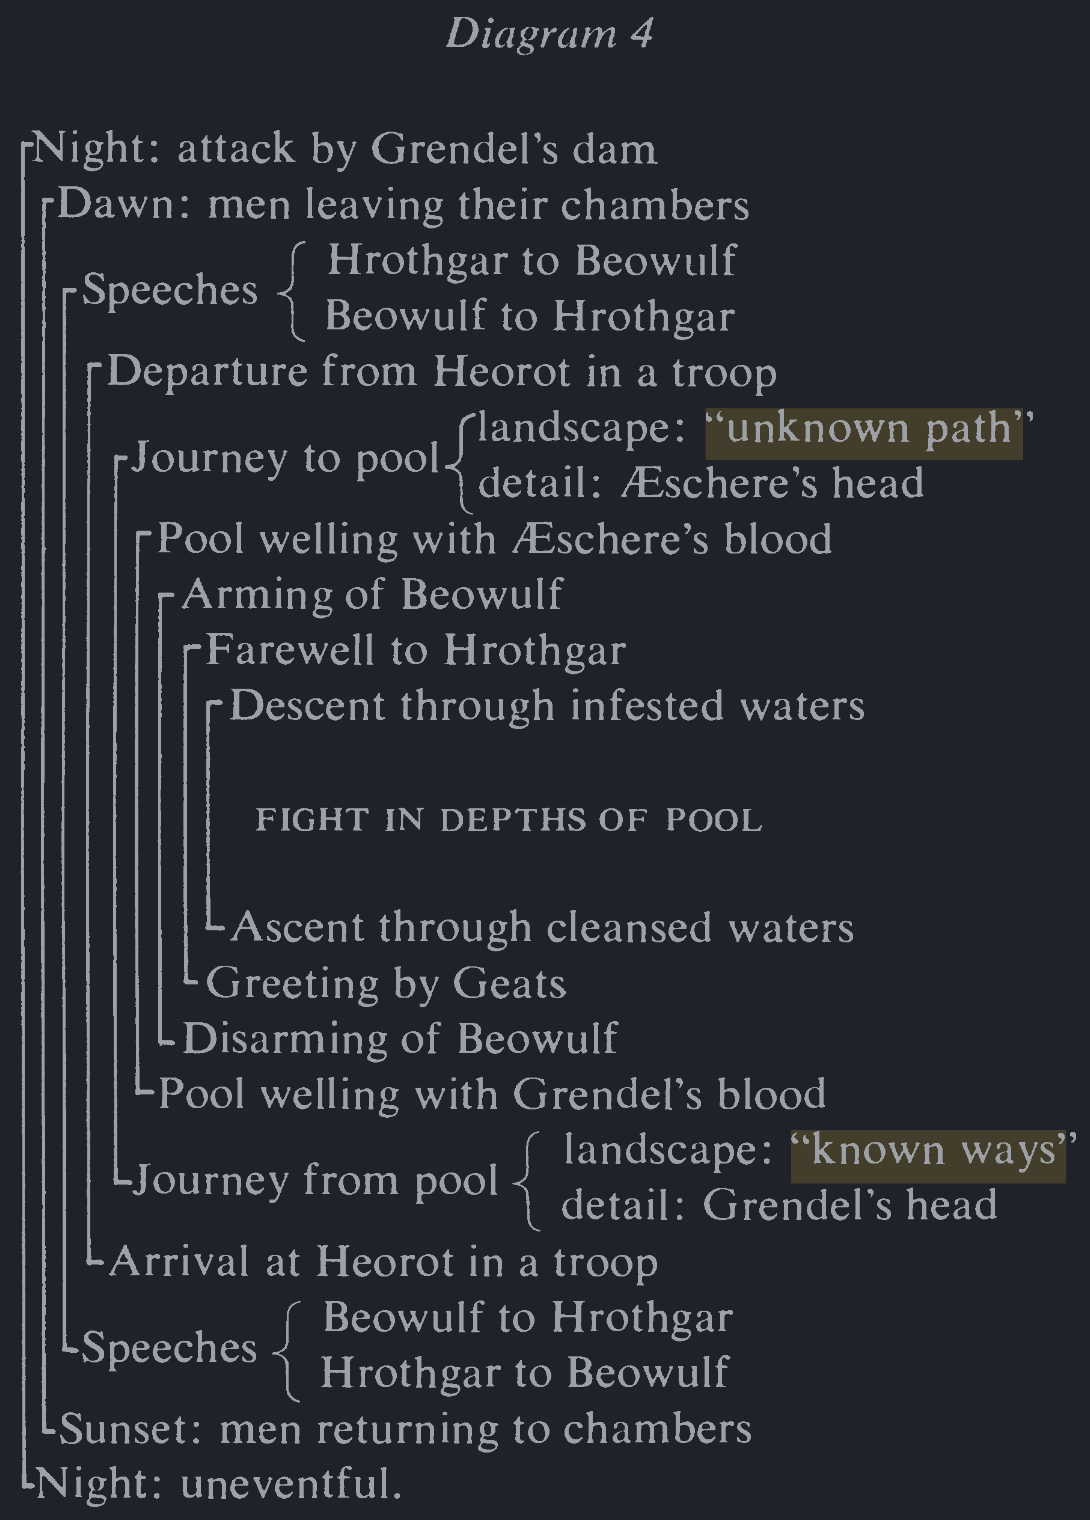
\includegraphics[width=\textwidth]{niles_diag4} 
    \end{column}

    \begin{column}{0.45\textwidth}
      \centering
      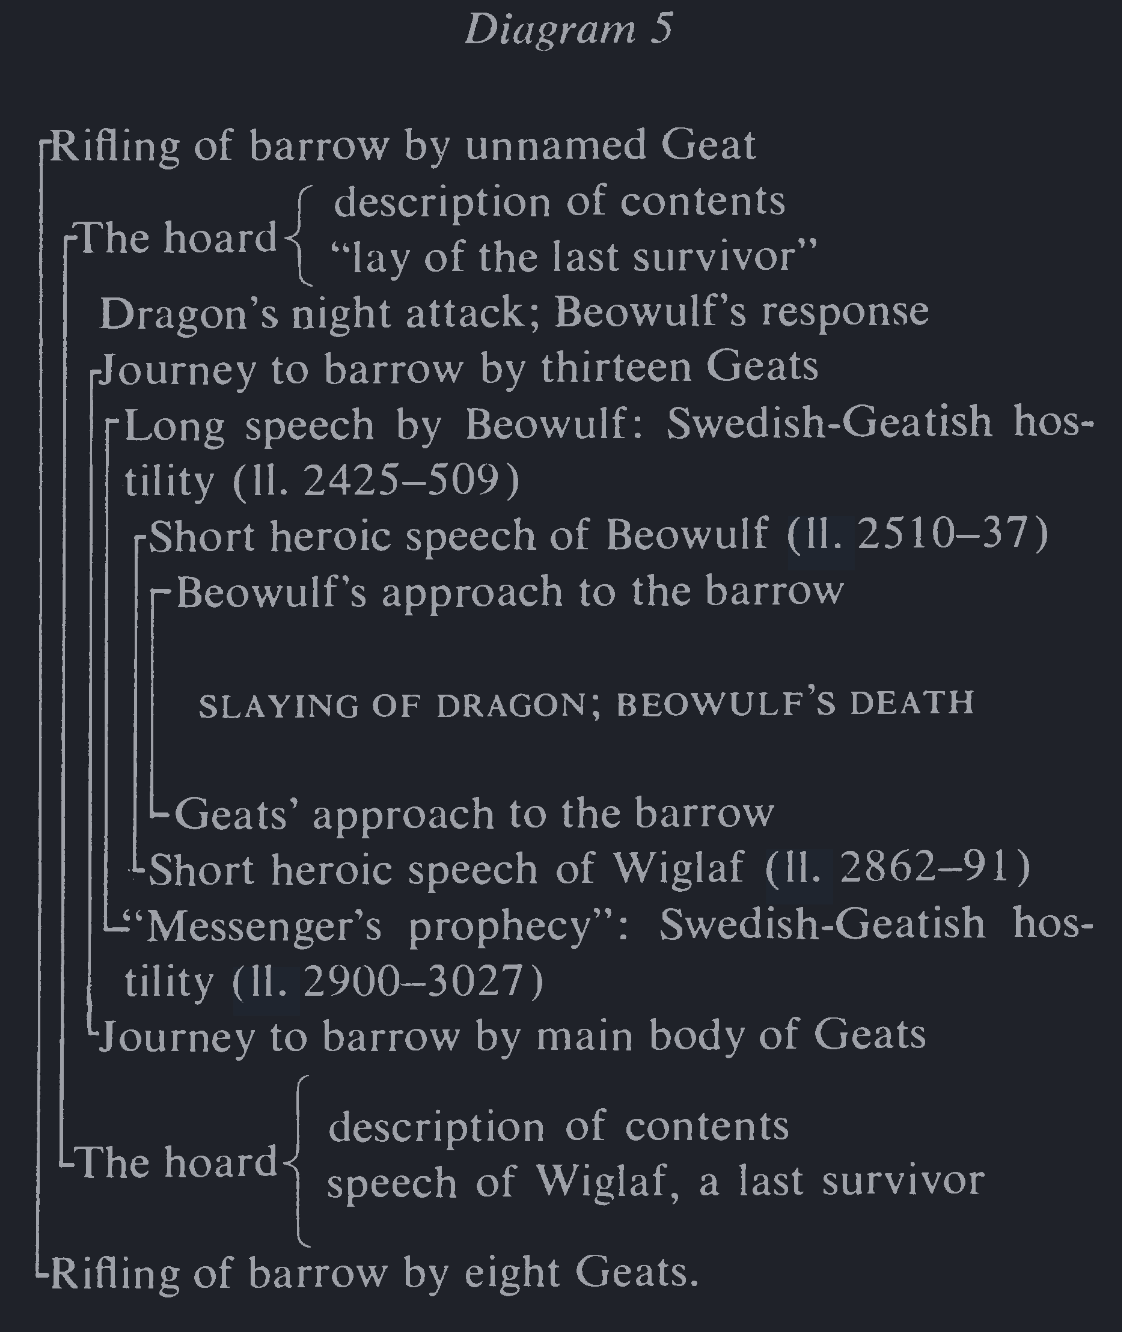
\includegraphics[width=\textwidth]{niles_diag5} 
    \end{column}
  \end{columns}
\end{frame}

\begin{frame}{Ring Composition: \textit{Beowulf}} 
  \begin{columns}[c]     
    \begin{column}{0.30\textwidth}
      \centering
      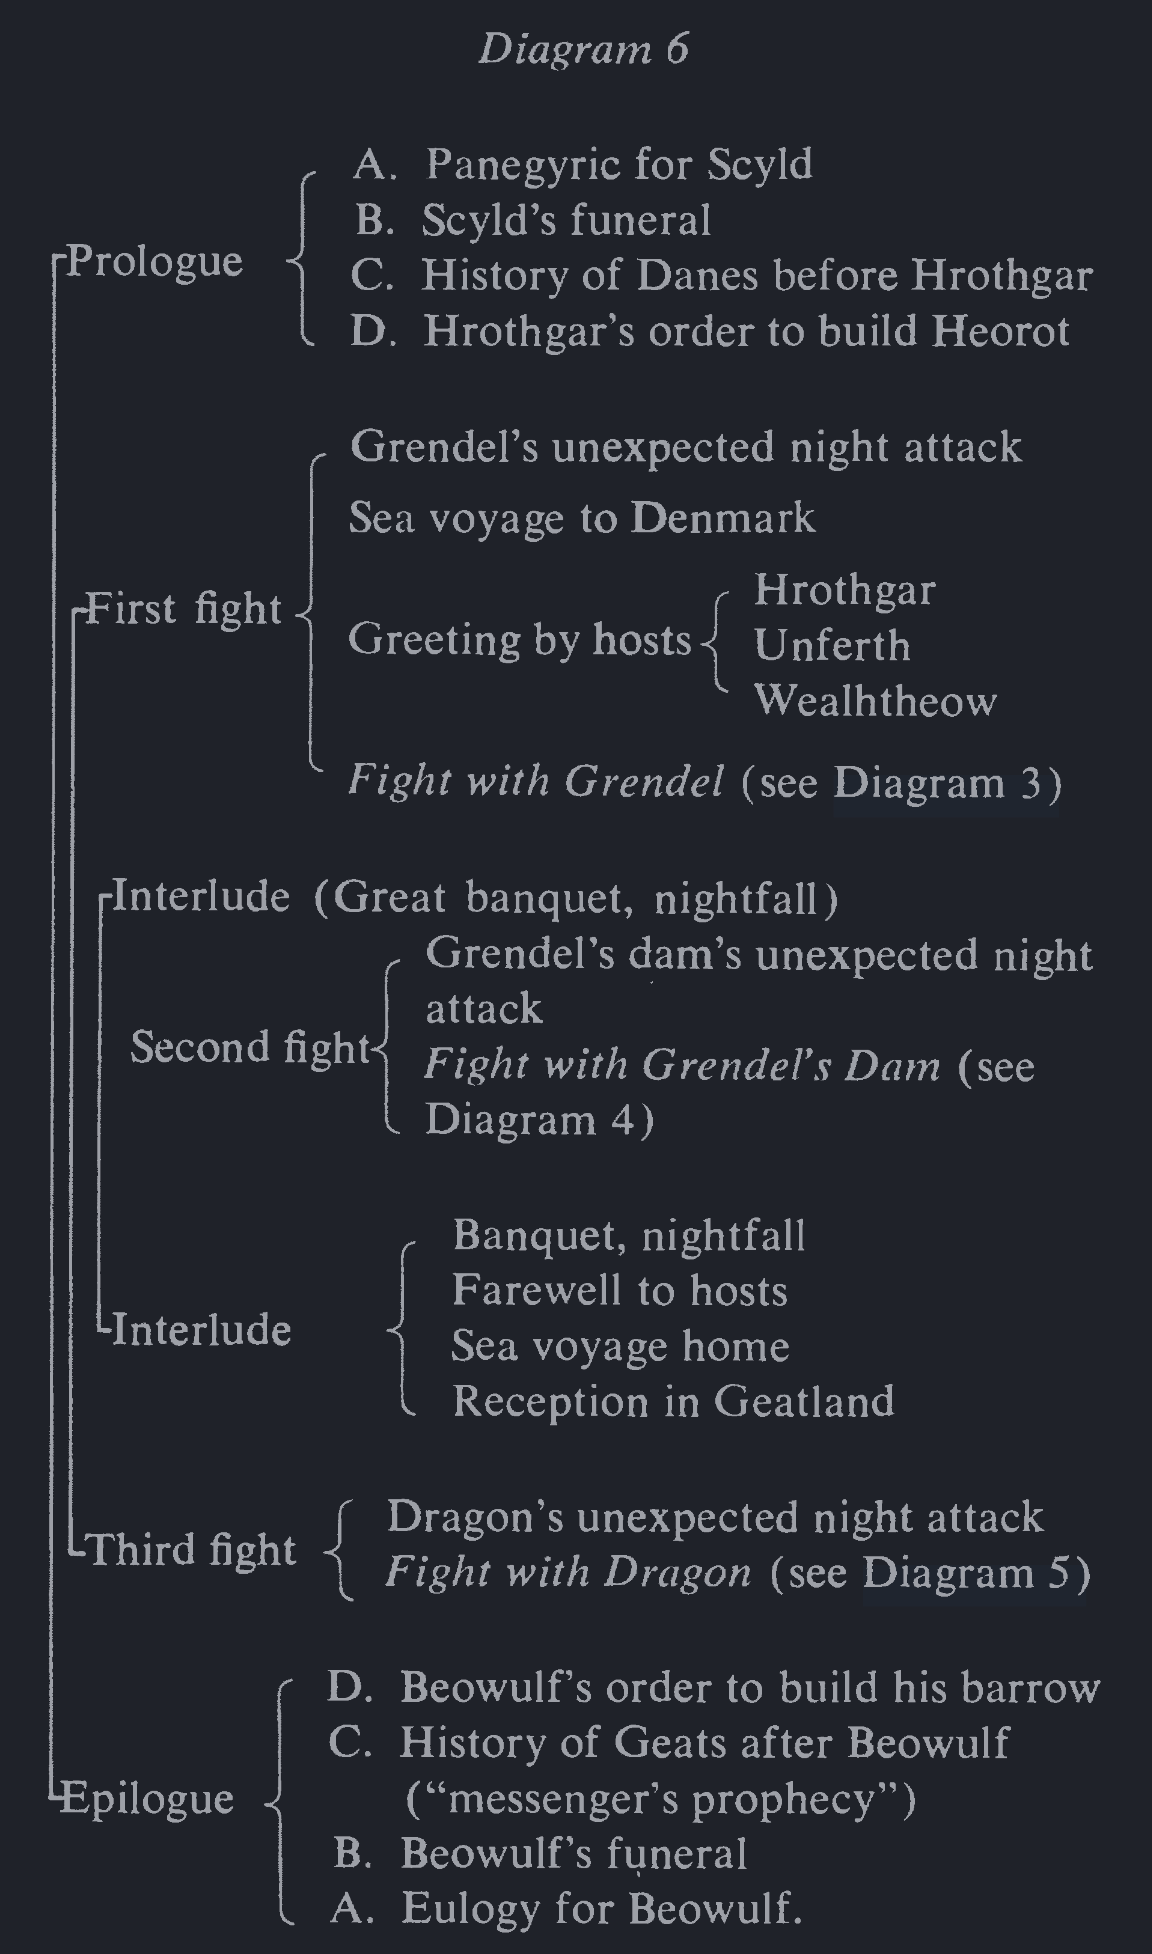
\includegraphics[width=\textwidth]{niles_diag6} 
    \end{column}

    \begin{column}{0.70\textwidth}
      ``In a way too consistent to be the result of chance, events in the poems' gradual unfolding find a reply in events from the poem's gradual close. 
      While these events are like one another in some ways, they are antithetical in others... \\
      ``In \textit{Beowulf}, it would appear, human success is and human failure are conceived as an inseperable pair... \\
      \onslide<2->{
        ``The poet, in fact, relied so heavily on this sort of patterning that for him balance and symmetry of thought must have been second nature" (Niles). 
      }
    \end{column}
  \end{columns}
\end{frame}

\begin{frame}{Criticism of Ring Composition Literature (Dane)}
  \begin{itemize}
    \item ``Neither the general nor the geometric form of ring composition can lead to convincing conclusion abouts about compositional practices beyond those that could be derived from the simple existence of specific repetitions." 
      \begin{itemize}
        \item e.g., Niles identifies an embedded theme as ``Grendel approaching" or ``phrase describing Beowulf." \\ 
          ``Such a ring surely owes its existence to critical rather than poetic viruosity" (Dane). 
      \end{itemize} 
    \item ``The entire notion of a frame is trivial and tautological: some sort of frame is logically implied in the very definition of a digression"
    \item ``The definition of the supposed phenomenon will in and of itself produce only positive evidence of the phenomenon." \\
      i.e., a constant or random sequence of motifs only provide \textit{neutral} evidence 
  \end{itemize}
\end{frame}

\newcommand{\mah}{\textit{Mah\={a}bh\={a}rata}\xspace}
\newcommand{\adi}{\textit{\={A}diparvan}\xspace}
\newcommand{\vai}{Vai\'{s}amp\={a}yana\xspace}
\newcommand{\jan}{Janamejaya\xspace}
\newcommand{\sarp}{\textit{sarpasattra}\xspace}
\begin{frame}{Epic Frame Story: \mah and \adi}
  Introduction to \adi: 
  \begin{itemize}
    \item ``This elaborate embedded tale of Cyavana, where one level of the story is interrupted to insert subordinate episodes, is evidently the result of lengthy historical growth"
    \item The first book of the \mah, a Sanskrit Epic about ``the passing of of the heroic age and the obliteration of the warrior race." 
      \\https://en.wikipedia.org/wiki/Mahabharata
    \item Primarily narrated by \vai to king \jan during the \sarp ritual  
      \begin{itemize}
        \item During intervals of recess during the ritual, \vai tells \jan about the history of the Bh\={a}rata 
      \end{itemize}
  \end{itemize}
\end{frame}

\begin{frame}{Epic Frame Story: \mah and \adi}
  ``The choice of the sarpasattra as the setting for the frame story of the Mahdbhdrata is a felicitous one for three reasons. 
  First, the theme of the destruction of the snakes, which is interrupted in time to save Taksaka, prefigures the fundamental theme of the epic it introduces
  -- the passing of the heroic age and the obliteration of the warrior race. 
  Indeed, it is the unborn Pariksit, saved by the special intervention of Krsna, who is the sole survivor of the epic era in the present age. 
  That Pariksit's killer, Taksaka, should be the one snake saved by special intervention from the flames of Janamejaya's sattra makes the two apocalyptic stories interlock" (Minkowski).

  \vspace{1em}
  But this ``interlock[ing]" relationship between \sarp and the main contents of \mah is a deliberate narrative device
\end{frame}

\begin{frame}{Epic Frame Story: \mah and \adi}
  ``The Mahabhdrata... provides itself with a sensible, well-structured frame story
  -- a long programmatic ritual session with regular intervals in the action set aside for talk, and a session, furthermore, that interlocks thematically with the epic it introduces" (Minkowski).

  \vspace{1em}
  The interlocking nature of the narrative induces embedded storytelling.
\end{frame}

\begin{frame}{Epic Frame Story: \mah and \adi} 
  ``If \vai is telling us the story of the Bh\={a}ratas, then who is telling us about \vai?"

  \vspace{1em}
  \onslide<2->{
    The \mah describes the ``history of its own narration" by adding a second narration that tells of the first :)

    The outer story is also narrated during a ritual. 
  } 
\end{frame}

\begin{frame}{Epic Frame Story: \mah and \adi}
  ``The sages' motivation in requesting the Bharata story is made evident. 
  The Bh\={a}rata story is the equal of the Vedas; 
  it is a Samhita composed by Vyasa. 
  Their interest, unlike Janamejaya's, is based on the ontological status of the epic, and not on the content of its main story" (Minkowski). 

  \vspace{1em}
  i.e., there is no need for another outer layer of narration
\end{frame}

\begin{frame}{Embedding Structure in \mah and \adi} 
  \begin{itemize}
    \item ``The embedded story must start after the story which embeds it. 
      One cannot append a substory at the beginning or end, outside its frame."
    \item `Linking passages' are highly formulaic:
        \begin{itemize}
          \item Audience established $\Longrightarrow$ narrator enters $\Longrightarrow$ hospitality $\Longrightarrow$ question to the narrator $\Longrightarrow$ request for more
          \item The lexical and morphosyntax used during these transitions are predictable
      \end{itemize}
  \end{itemize}
\end{frame}

\begin{frame}{Ritual and Epics} 
  \begin{itemize}
    \item Rituals often have recesses during which epics are told 
    \item Embedding structure in ritual: 
  \end{itemize}

  \begin{columns}[c]
    \begin{column}{0.5\textwidth}
      \centering
      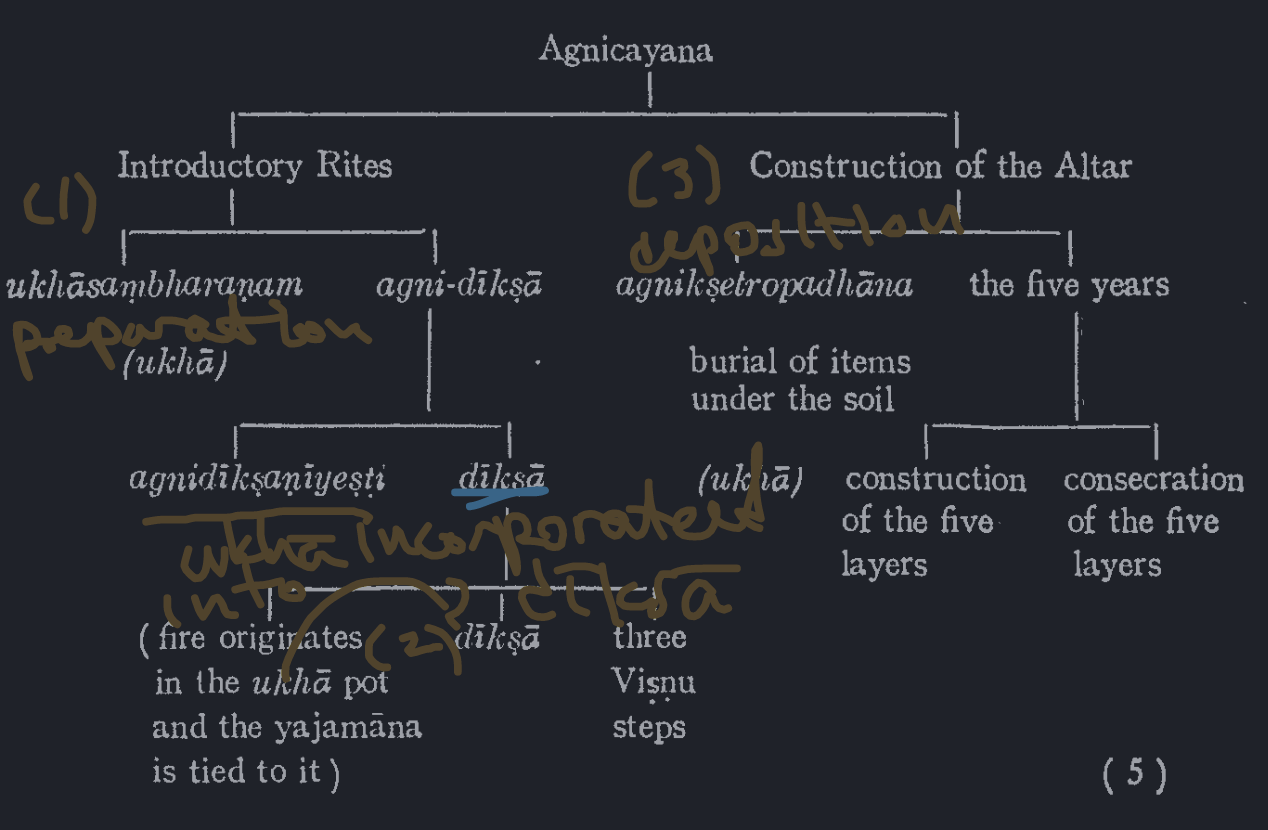
\includegraphics[width=\textwidth]{staal_ritsyntax} 
    \end{column}

    \begin{column}{0.5\textwidth}
      \centering
      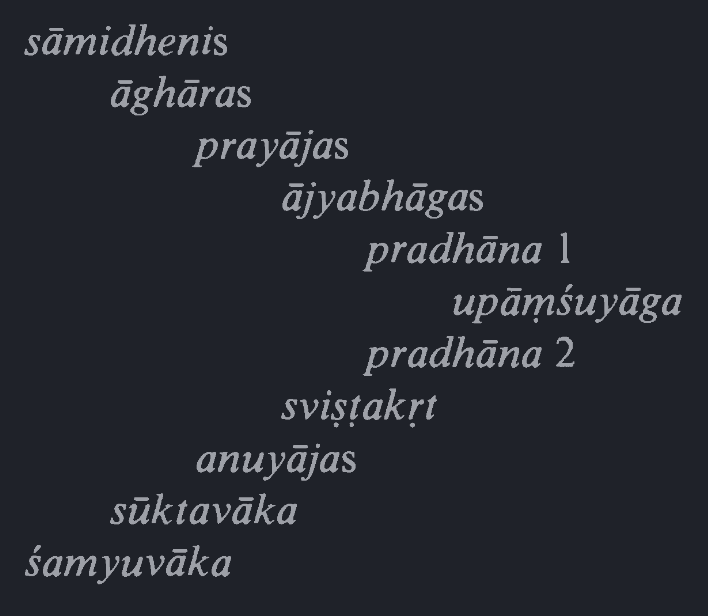
\includegraphics[width=\textwidth]{minkowski_ritsyntax} 
    \end{column}
  \end{columns}
\end{frame}

\end{document}
